% methodsandresults.tex

% Methods and Results
\section{Methods and Results}
\label{sec:methodsandresults}
We present the implementation of paravirtualized graphics acceleration in the Simics full-system simulator.
This method encompasses three overall components, being the target system libraries, the host system libraries, and a communications channel between them named the "Simics pipe".

For the purposes of ensuring scalability of the solution during development, we use code generation to produce the majority of target and host system libraries.
As such, the outmost majority of paravirtualized OpenGL functions are compiled by this tool.
The (\texttt{Python}) tool in question generates the OpenGL function definitions, on the sending and recieving end, from framework specification files detailing function signatures and argument attributes.
It generates all but the methods that require special treatment due to state saving.

The generated libraries, the Simics pipe, and implementation details thereof are presented in this section.

\subsection{Target System Libraries}
\label{sec:proposedsolutionandimplementation_targetsystemlibraries}
Compiled from \texttt{C} and \texttt{C++} sources output by the generation program, the target system libraries compose implementations of the EGL and OpenGL APIs.
Due to the tight coupling between OpenGL and the platform windowing system, the solution must also accelerate EGL -- the interface between OpenGL and the underlying platform windowing system.
As may be derived from the name, the target system libraries run on the simulation target.

The target system libraries implement the EGL and OpenGL~ES~$2.0$ APIs and lures whatever application it is being linked to that it is, in fact, the expected platform libraries.
Given that the target system libraries adheres to the OpenGL headers defined in the system, the application is na\"{\i}ve in terms of its paravirtualized status.
The interplay with the original OpenGL~ES headers also results in the solution adhering to the platform-dependent type definition, flags, and constants, as originally defined by Khronos.
However, instead of communicating with the platform windowing system (in terms of EGL) and the graphics device (in terms of OpenGL) -- and instructing said device in accordance to the user; the target system libraries serialize the given command stream and forward it to the simulation host.
However, the transmission of the command stream is not necessarily performed at once, or in the designated order, due to the formation of OpenGL.
This is because of uncertainties of the proportion of argument data, as size is not necessarily given by the user or apperent at that time.
As such, certain serialization may have to be delayed until further information surrounding the argument dimensions have been relayed to the OpenGL library.
Furthermore, a subset of the OpenGL state need be maintained by the target system libraries.
These attributes are comprised by, inter alia, bound vertex and index element buffers, in addition to properties of OpenGL vertex attributes.
Such states must be kept in the target system libraries due to the asynchronous nature of serialization of OpenGL invocations in the paravirtualized solution.

The serialization described in the above paragraph is thus formatted and encoded in accordance to a certain data format, which is kept as minimal as possible throughout execution.
The library on the target side packs data types of various lengths, such as $8$-bit characters, $16$-bit fields, or $64$-bit integer values, into fixed-length structures, so that the host system may interpret these values independently of how corresponding types are defined on that unrelated target platform.

%\footnote{It should be noted, however, that the solution assumes a little endian architecture and IEEE 754 standard for floating point representation. If the host system would not conform to these prerequisites, the solution would have to be complemented with additional support.}.

% Host System Libraries
\subsection{Host System Libraries}
\label{sec:proposedsolutionandimplementation_hostsystemlibraries}
In collaboration with the target system libraries, the host system libraries subsequently decodes and interprets the received byte stream.
Said decoding involves unpacking data from fixed length storage into variable-size types that OpenGL and EGL libraries expect.
Furthermore, and again similarly to the target system libraries, due to design inherent in the OpenGL~ES~$2.0$ framework, the host system libraries need to maintain some data for state saving purposes.
Such data is buffered in the host system libraries until used (drawn) in a later, and separate, OpenGL invocation.
%\footnote{A possible optimization would be to cache said data, to avoid the need to transmit unmodified vertices multiple times, despite so being specified by the user.}.
When the requested OpenGL invocation has been performed, any return or inout values are returned to the target system using the Simics pipe.
As with the the target system libraries, the receiving end of an OpenGL method definitions in the host system libraries are likewise generated to a large degree.

% Windowing Systems
\subsection{Windowing Systems}
\label{sec:proposedsolutionandimplementation_windowingsystems}
Due to variations in the creation and maintenance of windows on different platforms (Fedora, Android, etc.), the window to which OpenGL renders is kept on the simulation host.
This incurs the dilemma of the target system libraries having to communicate with the fraudelent window to which OpenGL renders in the simulation host, \textit{and} the native window, for example, reporting successful initialization.
After all, it would be problematic if the target OpenGL application would have to be modified in order to be paravirtualized.
Effectively, this means that it would be desirable to maintain the native functionality of the target system EGL library.
However, in order to swap the backbuffers to which OpenGL renders, one must use EGL.
In this way, the problem arises of a conflict between wanting to keep the functionality of the native EGL library, yet modify a small subset of it.
 
This issue is overcome by overriding symbols in the target libraries, effectively overloading desired functions, serialize and forward invocations to the host system, locate the next occurrence of the symbol in the symbol table, that is the original EGL function definition, and invoke the original function.
Accordingly, the target system EGL library does not replace the native target EGL library in its entirety, as with the OpenGL library, but rather extends it.
This gives the effect of a successfully created window, not having returned any errors in the window creation and maintenance -- yet having the application actually communicating with a different window.
As such, the target system libraries are effectively performing a man-in-the-middle attack on the target EGL library.

% Simics Pipe
\subsection{Simics Pipe}
\label{sec:proposedsolutionandimplementation_simicspipe}
The Simics pipe constitutes the target-to-host communications channel in Simics.
As such, it is responsible for transferring a serialized command stream between target software and simulation host.
In order to do this, the pipe requires a way to exchange information with the outside world.

There may be reasons why target software would like to escape the simulation and trigger that execution is resumed on the simulation host.
Such a scenario would be a debugging breakpoint, to share data between target and host systems, or for any reason modify the simulation state \todo{I don't understand this sentence}.
There are a number of ways to communicate with the outside world, including the host machine, from within the simulation, such as by networking means or specially devised kernel drivers, but few are as instant as "magic instruction".

\todo{This section has a lot of potential for trimming. As long as the reader is familiar with what a magic instruction means, we don't have to go into detail.}The magic instruction is a concept used to denote a \dvtcmdcodeinline{nop}-type instruction, meaning an instruction that would have no effect if run on the target architecture (such as \dvtcmdcodeinline{xchg ebx, ebx} on x86-compatible architectures), which, when executed on the simulated hardware in a virtual platform, invokes a callback-method in the simulation host~\dvtcmdcitebib[p.~32]{publications:leupers:2010}.
An advantage of this methodology is an often negligible invocation cost, as the context switch is often instant from the perspective of the target system~\dvtcmdcitebib[p.~131]{journals:rechistov:2013}.
Furthermore, being a greatly desirable attribute, magic instructions require no modification of the target system \todo{joho! magiska instr ar ju en modifiering av target, man andrar ju pa instruktioner. Syftar du pa att man inte behover lagga till latsashardvara? eller att mjukvara med MI aven funkar pa riktig HW? om det senare, sa ar detta orelevant for paravirtualisering}.
In effect, implementation of magic instructions requires replacing one or more instructions in the target instruction set, thereby making the magic instruction platform-dependent.
However, the solution is often designed to only respond to magic instructions wherein a certain magic number, sometimes called a 'leaf number'~\dvtcmdcitebib[p.~131]{journals:rechistov:2013}, is present in an arbitrary processor register.

Due to the inherent performance demands brought on by serialization of real-time graphics invocations, magic instructions are a suitable candidate for the exchange of information between target and host system.
Magic instructions allow for fast, in the pretext of the simulation target -- almost instant -- escape from the simulation context, and may carry a limited amount of information with it from inside the simulation out into the real world.
The role of the Simics pipe is comprised of the allocation and maintenance of page locked target memory to accomodate the use of magic instructions, which the Simics pipe uses to relay the starting address of said memory space to the simulation host.

During a magic instruction, values may be written to any registers fit for purpose; The number and size of processor registers is the data-sharing bottleneck of this method.
Not being the first time magic instructions have been used for the purposes of hardware acceleration~\dvtcmdcitebib[p.~32]{publications:leupers:2010}, the Simics Pipe utilizes such methodology, namely the \dvtcmdcodeinline{CPUID} x86 instruction, to carry a lone memory address, the starting address of the serialized command stream, in one of the target system registers.
The execution of the injected instruction in a simulated processor invokes a callback method in the host side of the Simics Pipe, having effectively escaped the simulation and paused the simulation state.
Knowing the occurrence of a magic instruction with the corresponding leaf number, the presence of a target virtual address in the agreed-upon CPU register may be assumed.
Note that, at this point, the retrieved address is in the format of a target system virtual address, the destination of which is unknown to the simulation host.
As such, this address need be translated in order to retrieve the package contents that the memory address points to.

\begin{figure}
\centering
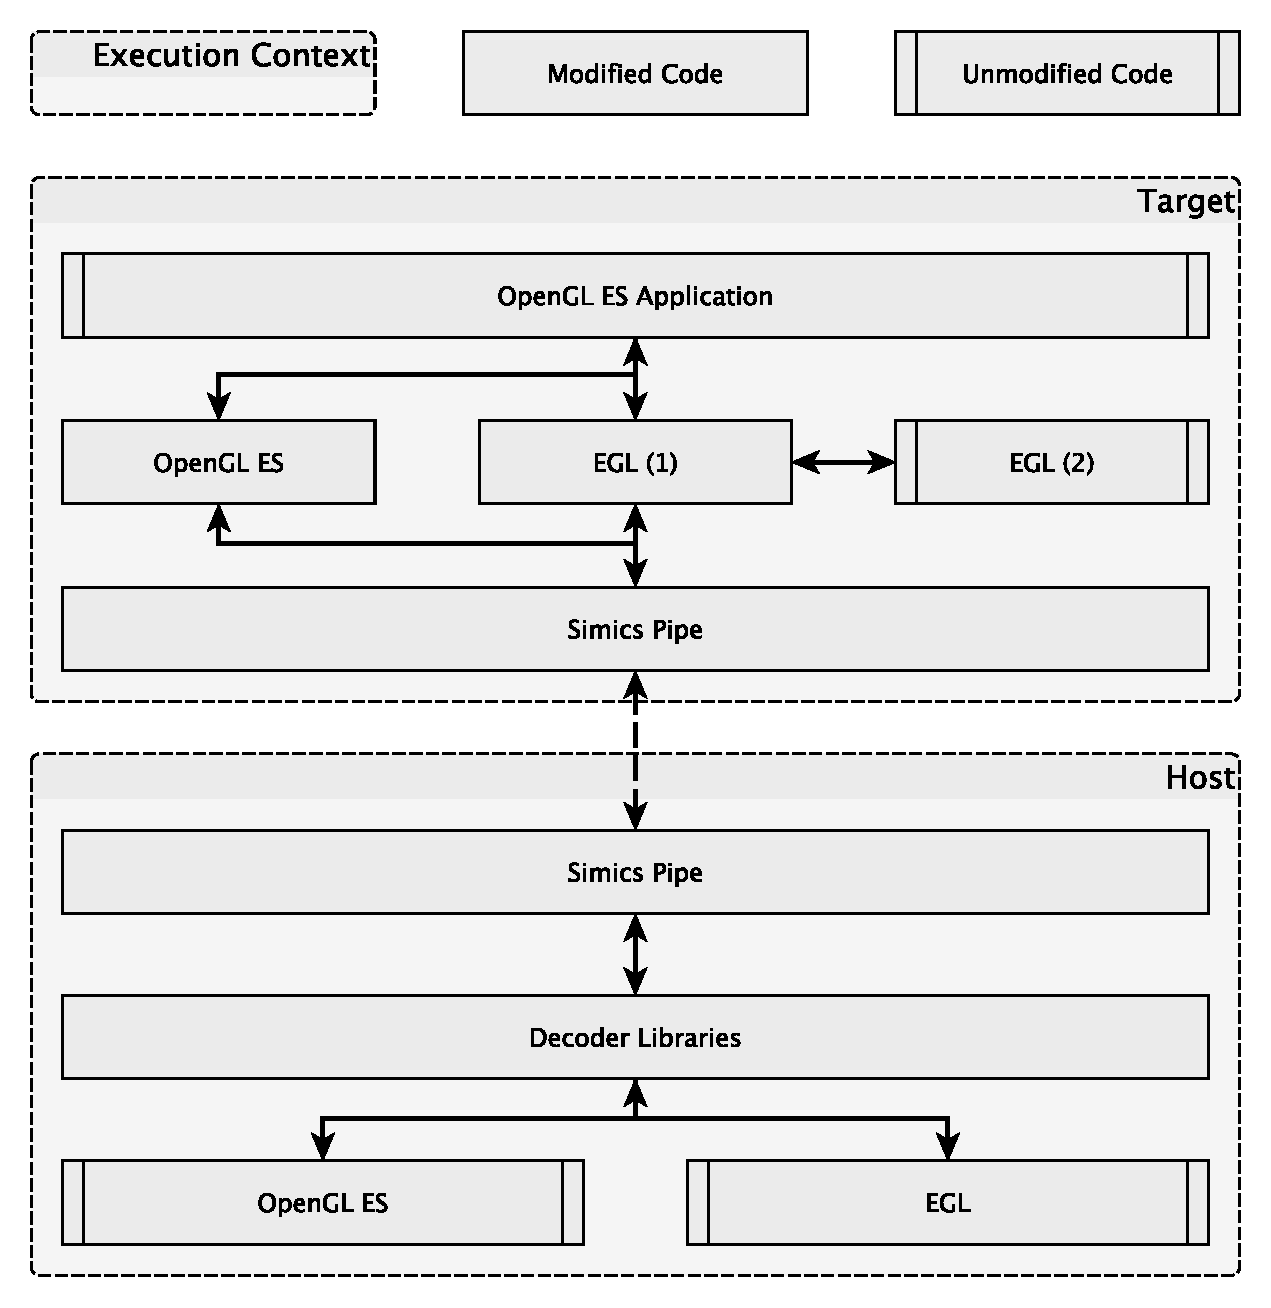
\includegraphics[width=\linewidth]{img/yedoverview.pdf}
\caption[Paravirtualization implementation overview]{Overview of the implementation accomodating paravirtualized graphics in Simics.}
\label{fig:overview}
\end{figure}

% Page Table Traversal
\subsection{Page Table Traversal}
\label{sec:proposedsolutionandimplementation_pagetabletraversal}
As outlined in section \ref{sec:proposedsolutionandimplementation_simicspipe}, target and host memory sharing is performed by the means of exposing a target virtual address to the simulation host.
The simulation host can access the MMU of the target system to translate a target virtual address to a target physical address.
The devised physical address can in turn be used to find the corresponding location in the simulated RAM image, thereby allowing direct access by the simulation host into the entire target memory page.
However, due to the complexity induced by circumventing the abstraction of virtual memory, there is no guarantee that the memory page to which the exposed physical address refers has not been swapped out of primary memory.
In order to solve this, the target system memory pages must be "locked" to prevent them from being swapped to disk.
This is the methodology used to ensure that the physical memory space, referred to by the virtual address sent to the simulation host, is still present in target primary memory when the simulation state is paused.
Other methods to achieve this include repeatedly 'polling' the corresponding memory pages in the target system.

Furthermore, and again induced by the unorthodox circumvention of the virtual memory paradigm, it is probable that the multiple memory pages making out particularly large serialized command streams, such as the transmission of vertex or texture data, are not consecutively aligned in physical memory, although guaranteed to be continuous blocks in terms of virtual memory.
As such, the physical addresses of memory pages must be continuously retrieved and translated on a per-page basis, effectively 'traversing' the virtual memory table (see Fig. \ref{fig:virtualmemory}).
This can be done in a trivial manner by simply iterating the original virtual address with the target page size.
In our case, the page size is $4096$ bytes.
Naturally, said process must be performed regardless whether data is being read or written.

\begin{figure}
\centering
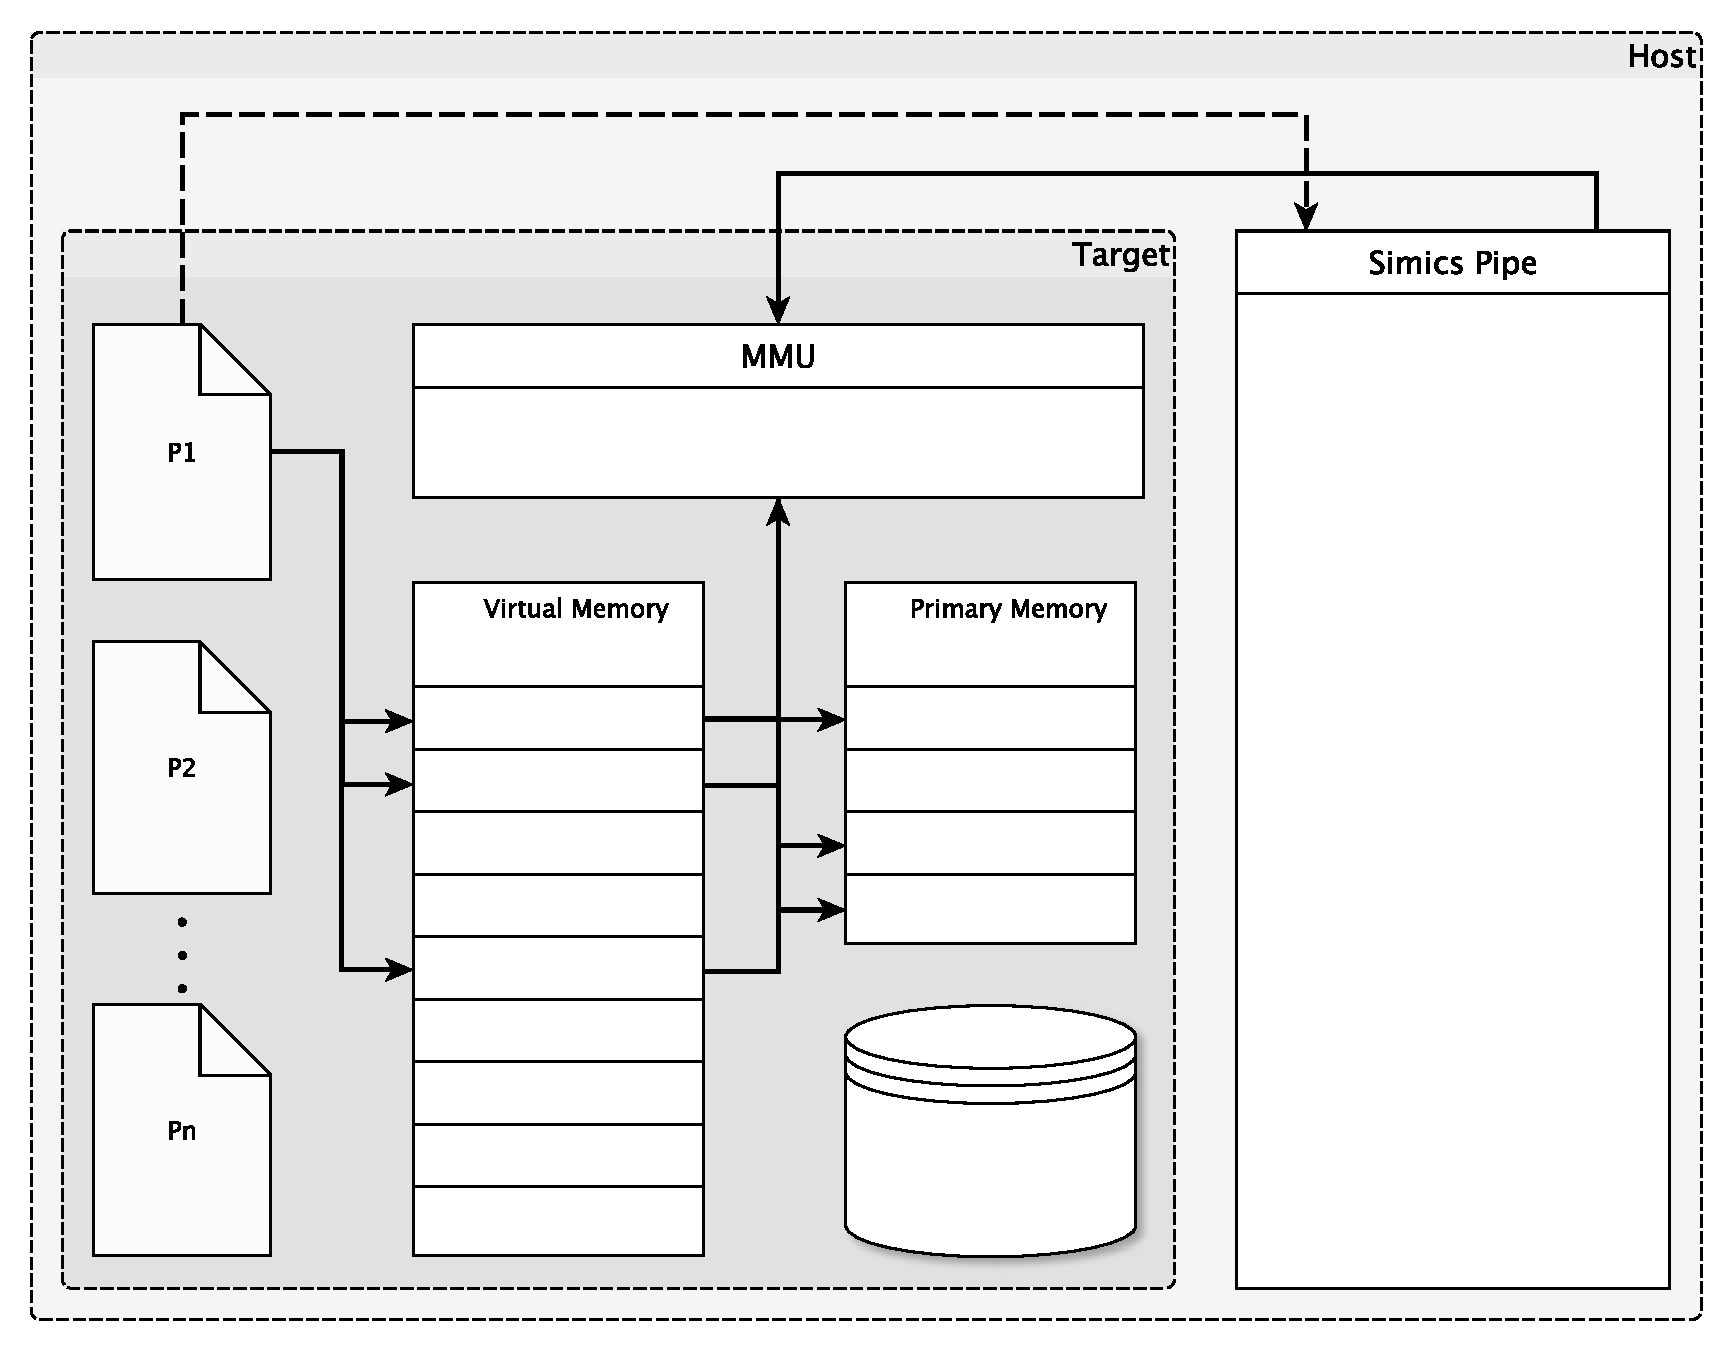
\includegraphics[width=\linewidth]{img/yedvirtualmemory.pdf}
\caption[Memory translation overview]{\hl{Memory translation overview. The OpenGL process hands a virtual memory address, pointing somewhere in the target system \textit{primary} memory, to the paravirtualized solution -- which inquiries the target system MMU to retrieve designated bytestream directly from target physical memory.}}
\label{fig:virtualmemory}
\end{figure}

\subsection{Experimental Methodology}
\label{sec:experimentalmethodology}
The experiments are performed in software rasterized and paravirtualized Simics platforms.
The results are compared to reference runs on the host system.
Simics is configured to simulate an Intel\circledR ~Core\texttrademark ~i7 processor.
During simulation, KVM\todo{Ref?}\ is used to  accelerate simulation by running target x86 instructions natively on the host hardware.
The simulation systems are, like the host system, set up to run Fedora $19$ Linux and use the Mesa llvmpipe driver\todo{Ref?}\ for OpenGL software rasterization.

The experiments are performed on a system running Fedora~19 Linux with the following specifications:
\begin{itemize}
\item Intel\circledR\ Core\texttrademark\ i7-4770HQ
\item Intel\circledR\ Iris\texttrademark\ Pro Graphics 5200
\end{itemize}

\todo{Motivate the development of your own benchmarks?}Two benchmarks are devised on-site for the purposes of stress-testing the paravirtualized technology described in this article.
Each benchmark is intended to stress one suspected bottleneck in the implementation: One benchmark performs a large number of relatively insignificant OpenGL invocations, while the other has a computationally intensive GPU workload.
Both benchmarks are configured to run at roughly $16$~\milli\second s per frame, which would correspond to roughly $60$~frames per second, when hardware accelerated on the host system.
The benchmarks are shaped this way in order to reflect the expected load of a modern real-time interactive application.
As such, the purpose of the benchmarks is to be representative of typical scenarios induced by modern graphics applications whilst utilizing a graphics framework such as OpenGL.
When run during the experiment, each benchmark instance measures the elapsed time of $1000$ frames.
Frame captures of the benchmarks are presented in Fig. \ref{fig:benchmarks}.

In order to further analyze how performance scales, we run three instances of each benchmark, using different input data.
In addition to the reference run of $16$~\milli\second , it is also run with smaller and larger input data, tuned to yield approximately half and double frame time, respectively, assuming that the benchmark really stresses the bottlenecks it was designed for.\todo{Elaborate}\
The specifics of the input data sizes are described below, along with the respective benchmark.

% fig:benchmarks
\begin{figure}
  \minipage{\linewidth}
  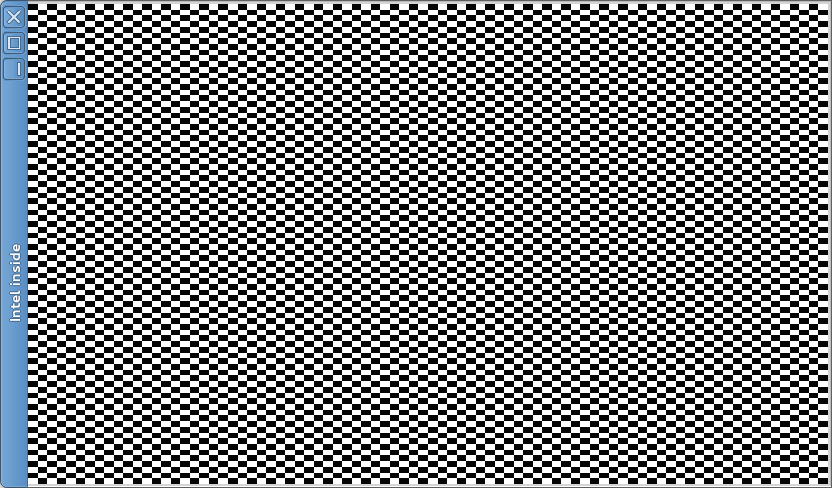
\includegraphics[width=\linewidth]{img/imgchess.png}
  \endminipage\\[6pt]
  \minipage{\linewidth}
  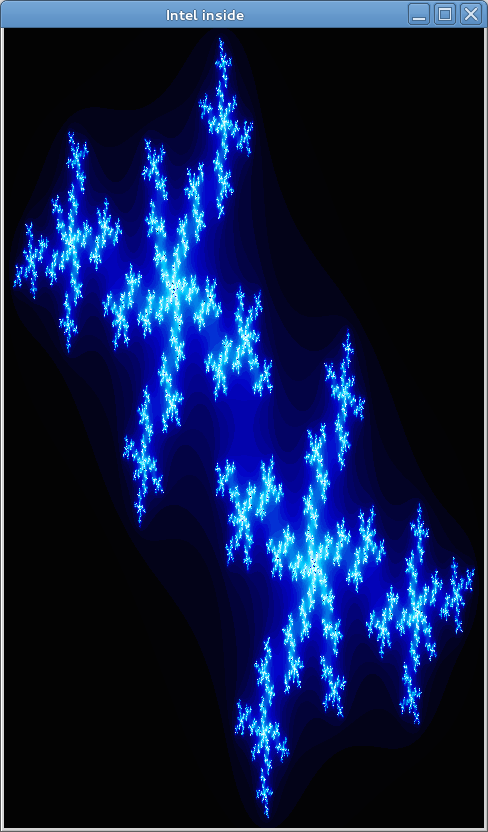
\includegraphics[width=\linewidth]{img/imgjulia.png}
  \caption[Benchmark screen captures]{Benchmark screen captures.}
  \label{fig:benchmarks}
  \endminipage
\end{figure}

% Benchmark: Chess
\paragraph{Benchmark: \hl{Chess}\todo{incorrect paragraph numbering}}
\label{par:experimentalmethodology_benchmarking_benchmarkchess}
\index{Chess benchmark}
The 'Chess' benchmark is developed for the purposes of stressing the latency between target and host systems.
It is so named because of the chess-like tileset the graphics kernel produces.
The benchmark is designed to perform a multitude of OpenGL~ES~$2.0$ library invocations per frame, in which each invocation is relatively lightweight in execution and carries a small amount of data in its arguments.
In the Chess benchmark, this is achieved by rendering a grid of tiles where each tile is represented by four two-dimensional vertices in screen-space, in addition to six indices outlining the rectangular shape.
Since the vertices are already transformed into screen-space, the graphics kernel need perform no additional transformation, adhering to the desired lightweight behavior of each kernel invocation.
Additionally, the tileset vertices and indices are pre-loaded into OpenGL vertex and index element buffers, so that a lone buffer identifier may be transferred instead of the heavier vertex set load.
Each tile is then individually drawn to the backbuffer, rendering the chess-like appearance of the benchmark.
Effectively, this means that, for each tile, the benchmark need only bind a vertex and an index element buffer, set the corresponding tile color, and lastly invoke the rendering of said tile.

For each frame rendered, depending on the number of drawn tiles, the solution will perform a large number of magic instructions.
This induces a high utilization of the Simics Pipe, which is intended to stress magic instruction overhead.
The repeated invocation of lesser draw calls is representative of common usage of drawing a multitude of shapes with OpenGL, such as a user interface. Additionally, the number of tiles being computed is easily modifiable, rendering the benchmark scalable for the purposes of the experiment described in this document. As such, said benchmark is considered suitable for the purpose of representing a large number of graphics invocations using OpenGL~ES~$2.0$.

We perform the Chess benchmark with $60\times60$, $84\times84$, and $118\times118$ tiles, which entails roughly $9\cdot60\cdot60$, $9\cdot84\cdot84$, and $9\cdot118\cdot118$ magic instructions per frame.
When profiled on the host system rendering $84\times84$ tiles, the Chess benchmark averages \dvtcmdfirstline{hostchess84x84.dat.avg} \milli\second .

% Benchmark: Julia
\paragraph{Benchmark: \hl{Julia}}
\label{par:experimentalmethodology_benchmarking_benchmarkjulia}
\index{Julia fractal benchmark}
The 'Julia' benchmark is developed for the purposes of stressing computational intensity in software-rasterized and paravirtualized platforms.
The kernel calculates the Julia fractal\todo{Ref?}, the texturing and frame-wise seeding of which gives the benchmark its distinct look.
The benchmark is designed to perform a lone computationally intensive graphics kernel invocation, which will stress the computational prowess of the profiled platform.
The case is selected for use as the computation of a fractal is trivially scalable in terms of complexity, by modifying the number of iterations the fractal algorithm performs, and is thus considered suitable for profiling of computationally intensive graphics kernels.

We perform the Julia benchmark with $225$, $450$, and $900$ iterations per frame, all of which induce $16$ magic instructions per frame.
Executed on the host system, the Julia benchmark induces an average frametime of \dvtcmdfirstline{hostjulia450.dat.avg} \milli\second .

\subsubsection{Platform Profiling\todo{strange numbering again}}
\label{sec:platformprofiling}
In the presence of complications caused by virtual time, profiling of elapsed time in simulators dictate special measures.
This is due to the fact that profiling of elapsed time outside of the simulation -- that is, time in the context of the observer -- may be more relevant than profiling of virtual time.
This is often the case if the simulation has outside dependencies of some sort.
Naturally, it is so in terms of real-time interaction and rendering.

In order to profile elapsed frametimes, profiling must take place outside of the simulation.
One way of achieving this is to listen in on activity passing through a target serial port; this is a traditional front-end to the machine.
In this way, the simulator is instructed to listen in on, and set a simulation breakpoint at the occurrence of, a specialized sequence of bytes being written (via a serial console) to a UART serial port.
This is the method we use to profile frametime performance in Simics.

When using serial ports in this manner, one may introduce a profiling cost.
Such overhead may be induced file descriptors not immediately transmitting a concerned byte sequence via the system UART.
We have measured this cost to be on average \dvtcmdfirstline{profile.dat.avg}~\milli\second , with a minimum and maximum elapsed time of \dvtcmdfirstline{profile.dat.min} and \dvtcmdfirstline{profile.dat.max}, respectively, adhering to a standard deviation of \dvtcmdfirstline{profile.dat.std}.
From these measurements, we may deduce that profiling overhead cost may occasionally be volatile.
However, with a standard deviation of \dvtcmdfirstline{profile.dat.std} \milli\second , slightly below that of the average, such large deviation is to be quite rare.
If not specified otherwise, all results have taken into account the average of this profiling cost, \dvtcmdfirstline{profile.dat.avg}~\milli\second .

\subsection{Results}
\label{sec:results}
Results accumulated from software rasterized and paravirtualized execution in Simics are presented in tables~\ref{tab:keyvalsimics}~and~\ref{tab:keyvalpara}.
In Fig.~\ref{fig:histogramssimicsparachess}~and~\ref{fig:histogramssimicsparajulia}, the results are presented as histograms, visualizing elapsed time in milliseconds to sample density.
As such, the $Y$ axis illustrate the sample density.
The histograms each feature $100$ bins, into which $1000$ samples, for each experiment performed \todo{unclear reference -- Do you mean that for each experiment, you put 1000 samples into 100 bins? maybe clearer if you split in 2 sentences}, are rounded into.
For the purposes of visualization, values outside of the standard deviation are not featured in the figures.
The remainder of this section presents an analysis of the data compiled from executing the experiment on the software rasterized and paravirtualized Simics platforms.

\providecommand{\chesskeyone}{$60\times60$ tiles}
\providecommand{\chesskeytwo}{$84\times84$ tiles}
\providecommand{\chesskeythree}{$118\times118$ tiles}

\providecommand{\juliakeyone}{$225$ iterations}
\providecommand{\juliakeytwo}{$450$ iterations}
\providecommand{\juliakeythree}{$900$ iterations}

\begin{table*}
  \parbox{.5\textwidth}{
    % tab:keyvalsimics
    \centering
    \begin{tabular}{|c|c|c|c|c|c|}
      \hline
      \multirow{2}{*}{Benchmark} & \multirow{2}{*}{Key} & \multicolumn{4}{p{4cm}|}{\centering Elapsed time (\milli\second )} \\
      \cline{3-6} && \multicolumn{1}{c|}{Min} & \multicolumn{1}{c|}{Max} & \multicolumn{1}{c|}{Std} & \multicolumn{1}{c|}{Avg} \\ \hline
      \multirow{3}{*}{Chess} & \chesskeyone & \dvtcmdfirstline{simicschess60x60.dat.min} & \dvtcmdfirstline{simicschess60x60.dat.max}	& \dvtcmdfirstline{simicschess60x60.dat.std} & \dvtcmdfirstline{simicschess60x60.dat.avg} \\ %\cline{2-6}
      & \chesskeytwo & \dvtcmdfirstline{simicschess84x84.dat.min} & \dvtcmdfirstline{simicschess84x84.dat.max} & \dvtcmdfirstline{simicschess84x84.dat.std} & \dvtcmdfirstline{simicschess84x84.dat.avg} \\ %\cline{2-6}
      & \chesskeythree & \dvtcmdfirstline{simicschess118x118.dat.min} & \dvtcmdfirstline{simicschess118x118.dat.max} & \dvtcmdfirstline{simicschess118x118.dat.std} & \dvtcmdfirstline{simicschess118x118.dat.avg} \\ \hline
      \multirow{3}{*}{Julia} & \juliakeyone & \dvtcmdfirstline{simicsjulia225.dat.min} & \dvtcmdfirstline{simicsjulia225.dat.max} & \dvtcmdfirstline{simicsjulia225.dat.std} & \dvtcmdfirstline{simicsjulia225.dat.avg} \\ %\cline{2-6}
      & \juliakeytwo & \dvtcmdfirstline{simicsjulia450.dat.min} & \dvtcmdfirstline{simicsjulia450.dat.max} & \dvtcmdfirstline{simicsjulia450.dat.std} & \dvtcmdfirstline{simicsjulia450.dat.avg} \\ %\cline{2-6}
      & \juliakeythree & \dvtcmdfirstline{simicsjulia900.dat.min} & \dvtcmdfirstline{simicsjulia900.dat.max} & \dvtcmdfirstline{simicsjulia900.dat.std} & \dvtcmdfirstline{simicsjulia900.dat.avg} \\ \hline
    \end{tabular}
    \caption[Benchmark results -- software rasterized in Simics]{Software rasterization benchmarking results in Simics.}
    \label{tab:keyvalsimics}
  }
  \hfill
  \parbox{.5\textwidth}{
    % tab:keyvalpara
    \centering
    \begin{tabular}{|c|c|c|c|c|c|}
      \hline
      \multirow{2}{*}{Benchmark} & \multirow{2}{*}{Key} & \multicolumn{4}{p{4cm}|}{\centering Elapsed time (\milli\second )} \\
      \cline{3-6} && \multicolumn{1}{c|}{Min} & \multicolumn{1}{c|}{Max} & \multicolumn{1}{c|}{Std} & \multicolumn{1}{c|}{Avg} \\ \hline
      \multirow{3}{*}{Chess} & \chesskeyone & \dvtcmdfirstline{parachess60x60.dat.min} & \dvtcmdfirstline{parachess60x60.dat.max} & \dvtcmdfirstline{parachess60x60.dat.std} & \dvtcmdfirstline{parachess60x60.dat.avg} \\
      & \chesskeytwo & \dvtcmdfirstline{parachess84x84.dat.min} & \dvtcmdfirstline{parachess84x84.dat.max} & \dvtcmdfirstline{parachess84x84.dat.std} & \dvtcmdfirstline{parachess84x84.dat.avg} \\
      & \chesskeythree & \dvtcmdfirstline{parachess118x118.dat.min} & \dvtcmdfirstline{parachess118x118.dat.max} & \dvtcmdfirstline{parachess118x118.dat.std} & \dvtcmdfirstline{parachess118x118.dat.avg} \\ \hline
      \multirow{3}{*}{Julia} & \juliakeyone & \dvtcmdfirstline{parajulia225.dat.min} & \dvtcmdfirstline{parajulia225.dat.max}	& \dvtcmdfirstline{parajulia225.dat.std} & \dvtcmdfirstline{parajulia225.dat.avg} \\
      & \juliakeytwo & \dvtcmdfirstline{parajulia450.dat.min} & \dvtcmdfirstline{parajulia450.dat.max} & \dvtcmdfirstline{parajulia450.dat.std} & \dvtcmdfirstline{parajulia450.dat.avg} \\
      & \juliakeythree & \dvtcmdfirstline{parajulia900.dat.min} & \dvtcmdfirstline{parajulia900.dat.max} & \dvtcmdfirstline{parajulia900.dat.std} & \dvtcmdfirstline{parajulia900.dat.avg} \\ \hline
    \end{tabular}
    \caption[Benchmark results -- paravirtualized in Simics]{Paravirtualization benchmarking results in Simics.}
    \label{tab:keyvalpara}
  }
\end{table*}

% fig:hostgramssimicsparachess
% fig:histogramssimicsparajulia
\begin{figure*}
  \centering
  \input{gnuhistogramssimicsparachess.tex}
  \caption[Benchmark results -- paravirtualized in Simics, Chess]{Histograms depicting benchmark elapsed frametimes in milliseconds and the density distribution of 1000 frames for the Chess benchmark key figure variations whilst software rasterized and paravirtualized in Simics. The $Y$ axis thus depict sample density. Its axis keys have been removed as they bear no relevance to the outcomes presented in this document.}
  \label{fig:histogramssimicsparachess}

  \input{gnuhistogramssimicsparajulia.tex}
  \caption[Benchmark results -- paravirtualized in Simics, Julia]{Histograms depicting benchmark elapsed frametimes in milliseconds and the density distribution of 1000 frames for the Julia benchmark key figure variations whilst software rasterized and paravirtualized in Simics. The $Y$ axis thus depict sample density. Its axis keys have been removed as they bear no relevance to the outcomes presented in this document.}
  \label{fig:histogramssimicsparajulia}
\end{figure*}

The data visualized in Fig. \ref{fig:histogramssimicsparachess} shows that the Chess benchmark, when software rasterized in Simics, has a broad sample density distribution, yet the distribution seem evenly distributed around a single point.
The right-hand side of the graph, while also showing impaired performance induced by paravirtualization, visualize a decrease in sample density distribution.
This is supported by the data presented in table \ref{tab:keyvalpara}.

Based on the data summarized in table \ref{tab:keyvalsimics} and comparing said data to that of table \ref{tab:keyvalpara}, we may observe that the software rasterized solution outperforms its paravirtualized counterpart, regardless of number of tiles rendered.
% When comparing these results to the uncompromised hardware accelerated counterpart on the host machine (see Fig. \ref{fig:histogramshost}), we may observe - albeit considerably less prominent - an adherence to the single-peak behavior in the distribution of the sample density.

The Chess benchmark is designed to locate any bottlenecks related to the number of paravirtualized invocations, which was predicted a bottleneck..
Evidently, the prediction of a target-to-host communication letency issue has been confirmed, arguably identifying one weakness of graphics paravirtualization in the Simics full-system simulator.

\todo{Elaborate on your non-VMP findings here.}In Simics, magic instructions incur a context switch cost when exiting the simulation and beginning execution on the host.
This affects the performance by forcing the simulation to no longer be executed in native mode, inhibiting the simulatory performance improvements granted by hardware-assisted virtualization.
It also entails Simics no longer being able to utilize just-in-time compilation to speed up execution, having to rely on regular code interpretation.
As such, in great numbers, magic instructions may greatly affect performance.

In order to establish what those overhead costs may be, further study into this matter is performed.
To do this, elapsed time for escaping simulation $1000$ times using magic instructions is measured, collecting minimum (\dvtcmdfirstline{magicinstrprofileall.dat.min}~\milli\second ), maximum (\dvtcmdfirstline{magicinstrprofileall.dat.max}~\milli\second ), average (\dvtcmdfirstline{magicinstrprofileall.dat.avg}~\milli\second ), the standard deviation thereof (\dvtcmdfirstline{magicinstrprofileall.dat.std}~\milli\second ), time to do so \todo{kan meningen forenklas lite? lite val komplexa syftningar}.
From these findings, we may conclude that the execution of $1000$ magic instructions is expected to induce an average overhead of \dvtcmdfirstline{magicinstrprofileall.dat.avg}~\milli\second  per magic instruction.
Indeed, these findings indicate that magic instruction overhead could very well account for the majority of the elapsed average frametimes when paravirtualized in Simics.

In Fig. \ref{fig:histogramssimicsparajulia}, we may observe double to triple peak behavior in the distribution of the sample density, both in software rasterized and paravirtualized platforms.
What causes this behavior is unclear, as frame-to-frame branching in the fractal algorithm is minor and ought not cause such a variance.

The Julia benchmark is incorporated into the experiment to establish how the paravirtualized solution performed under computational stress, which is where benefits induced by hardware acceleration should be made apperent.
Using this benchmark, we highlight weaknesses in Simics software rasterization, with frame times well above the two second mark; the corresponding maximum frame time in the paravirtualized Simics platform measuring up to to a mere \dvtcmdfirstline{parajulia900.dat.max} \milli\second .
As visualized in Fig. \ref{fig:histogramssimicsparajulia}, we showcase considerable performance improvements and -- in turn -- identify the capabilities of graphics paravirtualization in the Simics full-system simulator.

% Albeit the hardware accelerated host profiling (see Fig. \ref{fig:histogramshost}) may, however minor, suggest such a pattern; it is by all means not significant.
% We may observe similar behavior in the distribution of the sample density when profiling the same benchmark whilst paravirtualized in the QEMU -derived Android emulator (see Fig. \ref{fig:histogramsqemu}).

%% % Platform Comparison
%% \subsubsection{Platform Comparison}
%% \label{sec:analysisexperiment_platformcomparison}
%% \todo{This sections should be moved or removed depending on whether or not we bring up QEMU.}
%% In the sections above, results have been presented indicating performance gains, and potential for gains, in Simics platforms by the means of accelerating graphics using paravirtualization.
%% However, in accordance to Fig. \ref{fig:histogramsqemu} and table \ref{tab:keyvalqemu}, the platform on which the these results have been produced also utilizing paravirtualized methodology, there is much potential for improvement.
%% The benchmarks, when executed in the paravirtualized Android emulator, exhibit better performance in each test performed for the purposes of this paper; most notably outperforming the software rasterized Simics platform for the Chess benchmark.
%% The Chess benchmark, incurring such an overhead when paravirtualized in Simics (see paragraph \dvtcmdrefname{par:results_chess}) due to overhead induced by magic instructions (see section \ref{sec:results_magicinstructionoverhead}), performs but roughly two times worse than its hardware accelerated counterpart at \dvtcmdfirstline{qemuchess84x84.dat.avg} \milli\second  average (see tables \ref{tab:keyvalqemu} and \ref{tab:keyvalhost}).
%% These results indicate potential for improvement in the target -to-host communications in Simics.
%% In fact, considering the large similarities in the paravirtualized methodology for graphics acceleration these two platforms share, the reference performance of the QEMU -derived Android emulator may be considered a goal for a potential productification of paravirtualized graphics in the Simics full-system simulator.

%% These comparisons suggest that the recorded performance for the benchmarks, devised for the purpose of this study, is not necessarily representative for paravirtualized graphics in general.
%% Furthermore, the comparison to the QEMU -derived Android emulator indicates that the shaping of the magic instruction -utilizing Simics Pipe - as established being the bottleneck during execution of the paravirtualized Chess benchmark (see section \ref{sec:results_magicinstructionoverhead}) - may have potential of improvement of approximately one order of magnitude (see tables \ref{tab:keyvalqemu} and \ref{tab:keyvalpara}).

%% Based on the reference profiling presented in Fig. \ref{fig:histogramshost}, we may conclude that the benchmarks, when hardware accelerated on the host system, perform with concentrated density; not being much scattered across the graph except a few irregular extremities in terms of maximum frame times (see table \ref{tab:keyvalhost}).
%% This is supported by the standard deviation presented in said table.
%% Furthermore, we may conclude that the Phong demo features two distinct peaks in density distribution - about $1$ \milli\second  in-between.
%% There may be cause to believe that this is caused, or partly caused, by frame-wise rotation of the teapot - rotation featured in the benchmark (see section \ref{sec:experimentalmethodology_benchmarks}) - inducing some fluctuation into its execution (see Fig. \ref{fig:histogramssimicsparaphong}).
%% However, this behavior is, strangely so, not apparent whilst paravirtualized in the QEMU derived Android emulator, although this may be a visual artifact due to the resolution of the graph (see Fig. \ref{fig:histogramsqemu}).
%% See section \ref{sec:threatstovalidity_benchmarkvariations} for an elaboration on divergence in the Phong benchmark.
%% Additionally, and in accordance to tables \ref{tab:keyvalhost} and \ref{tab:keyvalqemu}, one may observe relatively high recorded maximum frame times in relation to compiled maximum- and average values, yet featuring - in relation to divergent maximum, relatively low standard deviations.
